\chapter{Simulations over ER and BA networks, plus a failed attempt on SW}

\resp{Vicentini Gioele}

For all the networks the strategy is the same: first generate two copies of the network, then apply q-swap of degrees $2,3$ to one of the two copies, to then finally study their behavior under bond percolation. The results for ER and BA networks are in \autoref{fig:ER_BA_perc}. BA networks are famous for being robust under bond percolation, so while the effect of $2,3$ swaps is still present, it's less relevant. This proves how much the underlying topology of the network is relevant when designing processes apt to enchance specific qualities of the network.

\begin{figure}
    \centering
    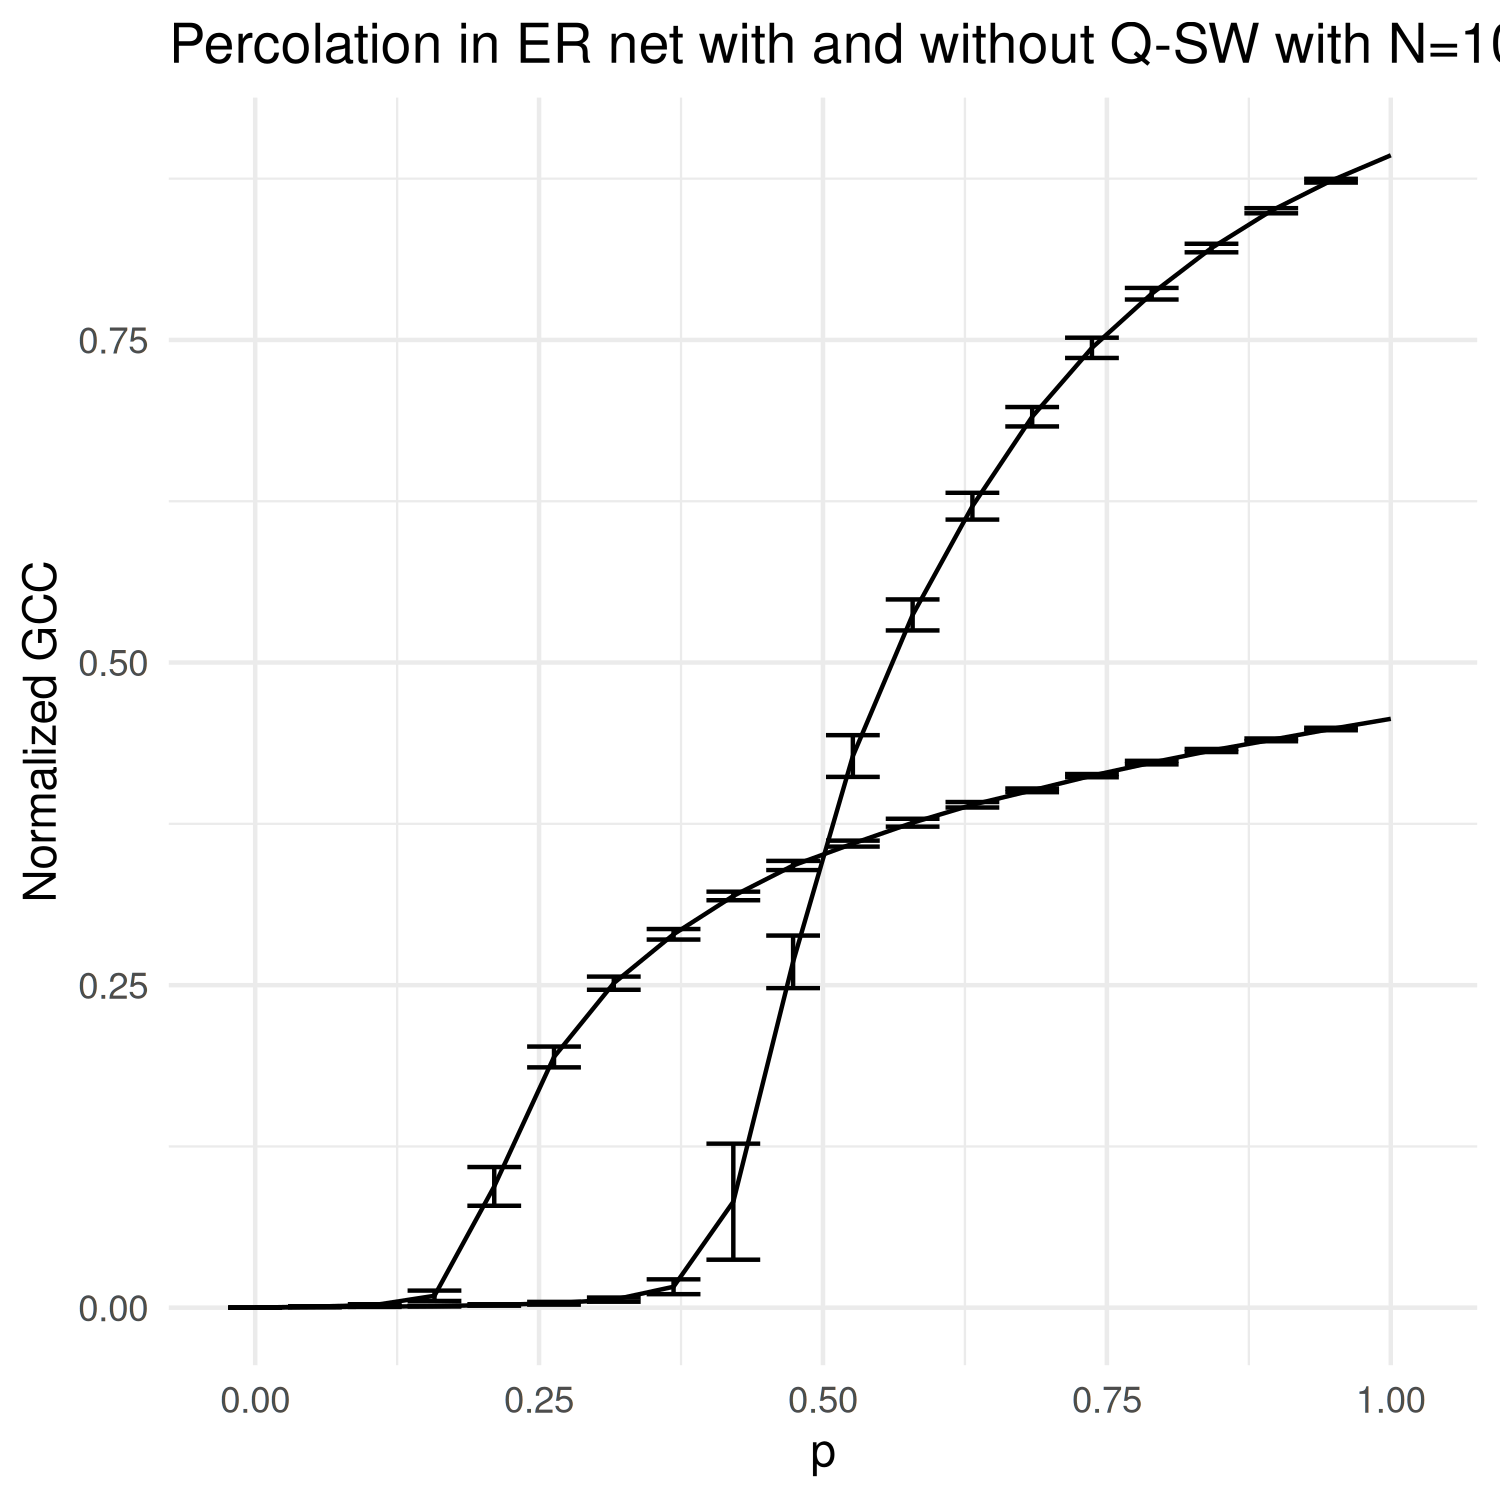
\includegraphics[width=0.45\linewidth]{images/ER_perc_10000.png}
    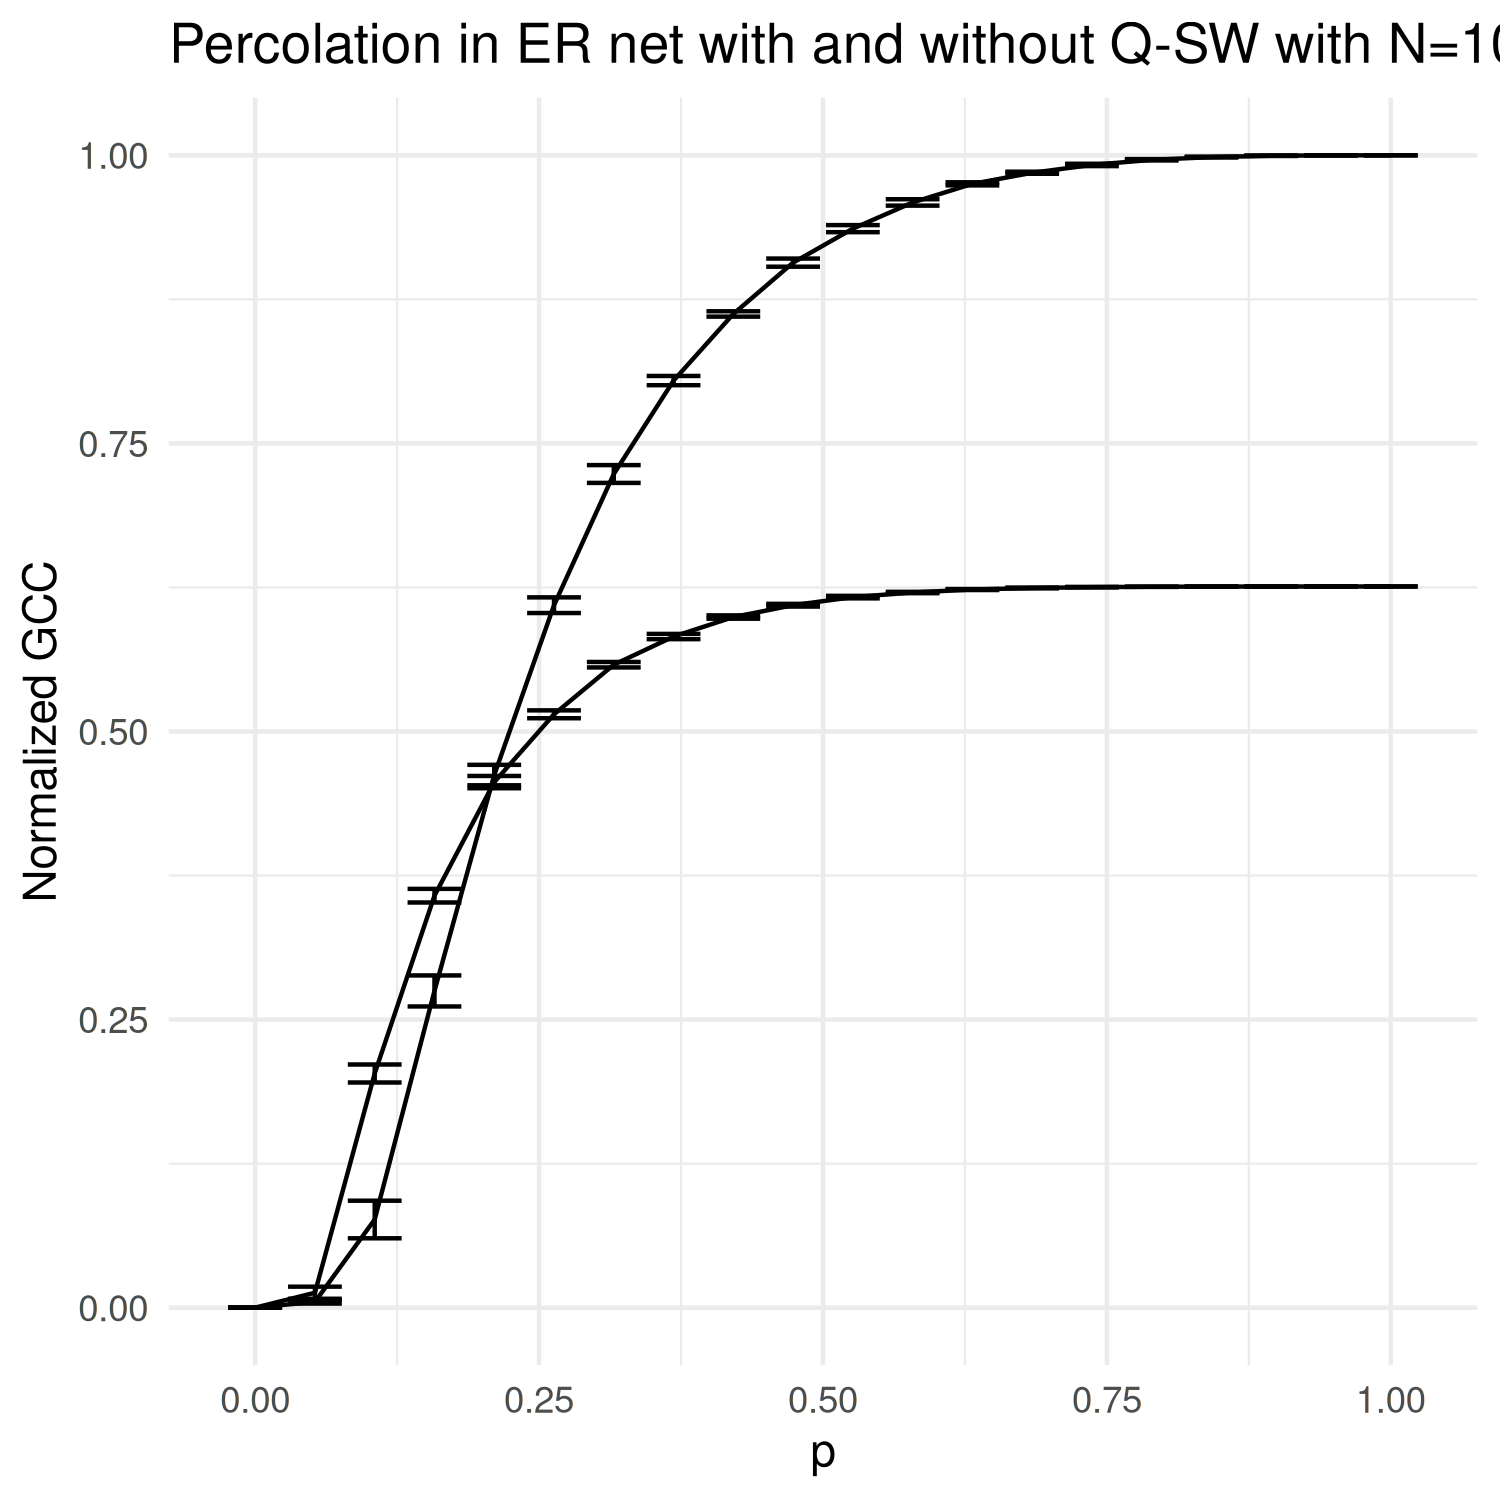
\includegraphics[width=0.45\linewidth]{images/BA_perc_10000.png}
    \label{fig:ER_BA_perc}
    \caption{Results of simulations of robustness against bond percolation. Left: ER network of $10^4$ nodes with avg. degree $2.5$. Right: BA network of $10^4$ nodes with $3$ edges added per timestep. As expected, BA networks are more robust under bond percolation and the $2,3$ swaps are not so relevant.}
\end{figure}
 
In \autoref{fig:SW_perc} there's a failed attempt of replicating Figure $3.b$ of the paper, where percolation and q-swappings are applied on a Small World network with added shortcuts. Due to the limited computational power available, the network studied here is relevantly small, $N\sim 10^3$, which means that the added edges are less than what studied in the paper ($N\sim 10^6$), although the addition probability is higher ($0.5$ against $0.25$).
\begin{figure}
    \centering
    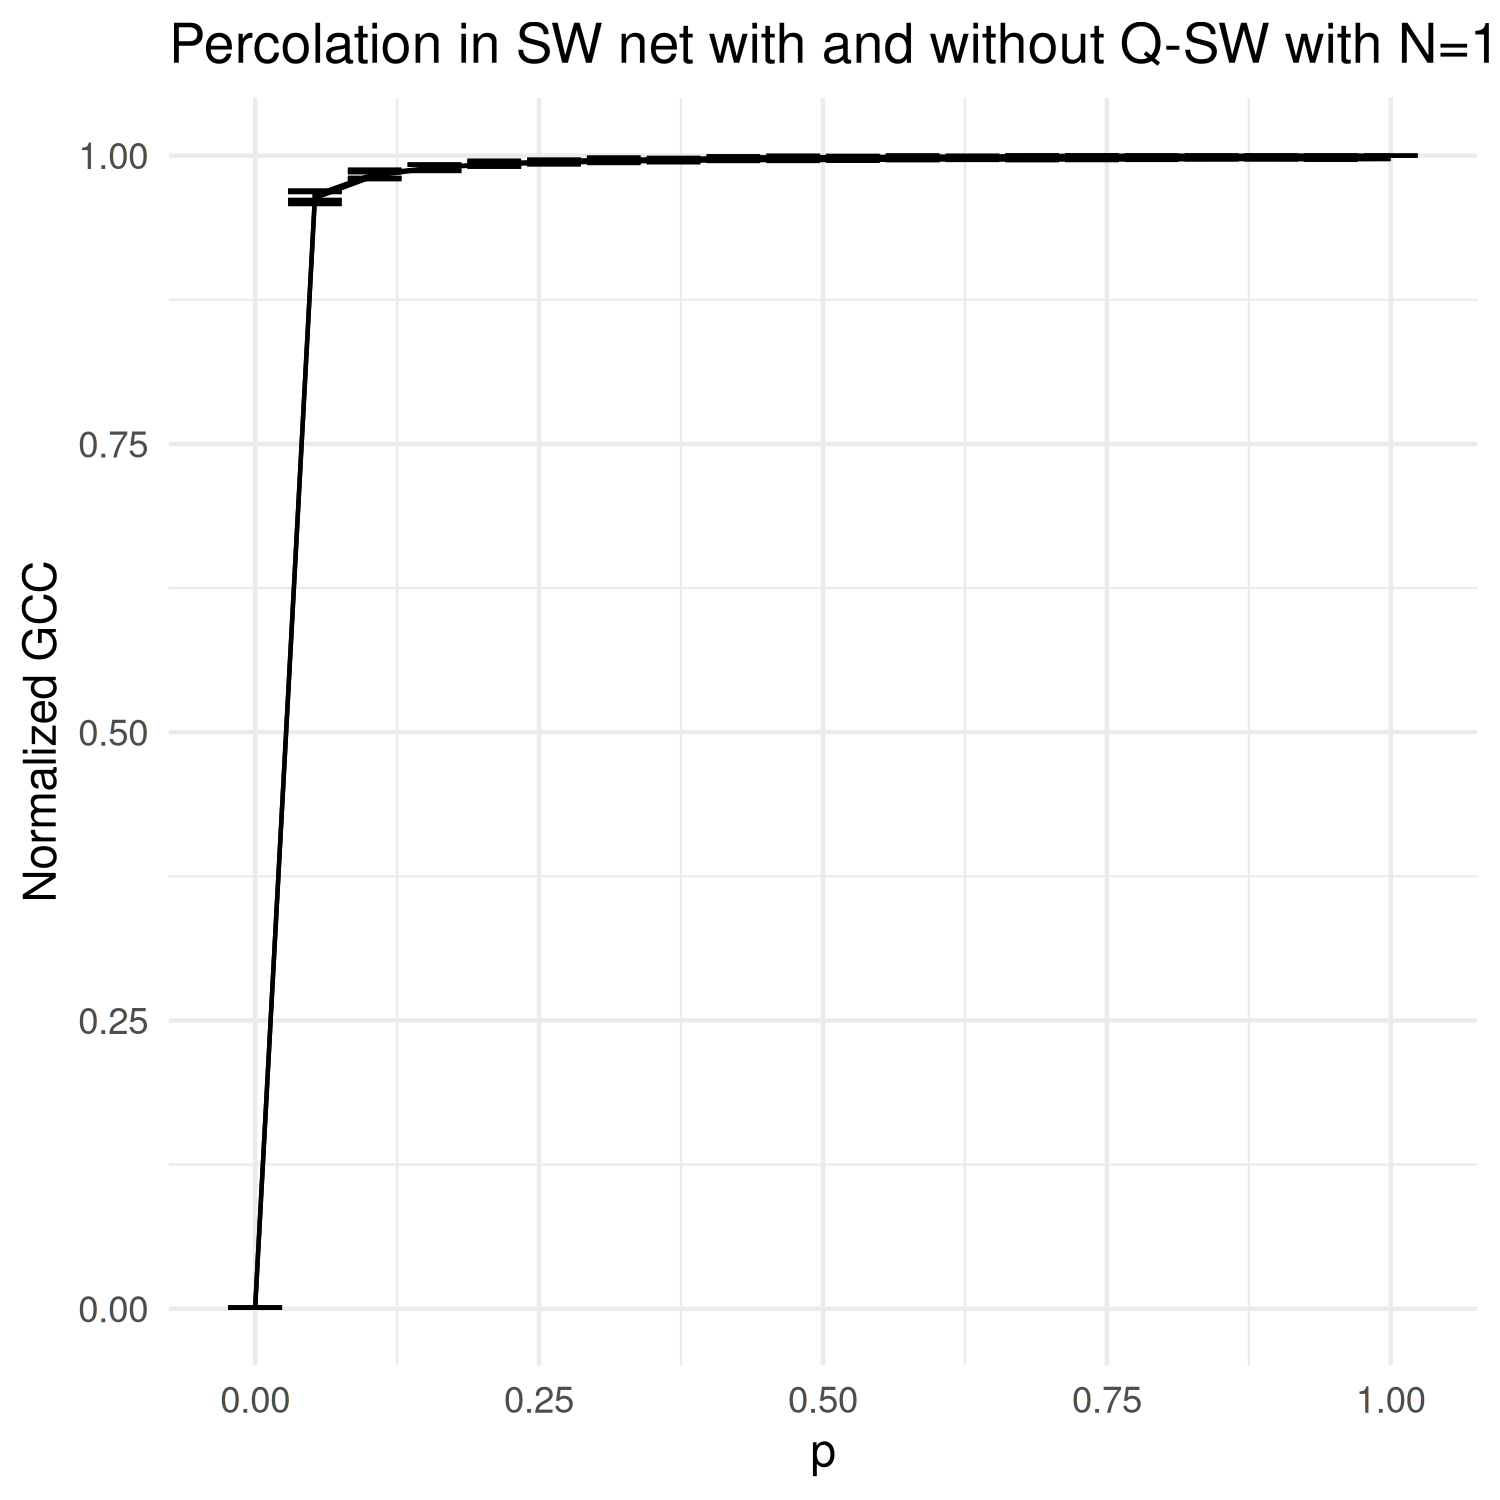
\includegraphics[width=0.45\linewidth]{images/SW_perc_1000.png}
    \label{fig:SW_perc}
    \caption{Bond percolation after $2,3$ swap on a Watts-Strogats Small World model with $10^3$ nodes and shortcut addition probability $\phi=0.5$. As expected of such highly redundant networks, neither percolation nor q-swaps have relevant effects.}
\end{figure}

\newpage